\begin{frame}[fragile]
  \pdfnote{IoT besteht aus vielen Dingen}
  \pdfnote{Smartphones, Kühlschränke, Schlösser, Autos...}
  \pdfnote{Marius hat eine smarte Waage}
  \pdfnote{Patrick sein Rad "smart gemacht"}
  \begin{center}
    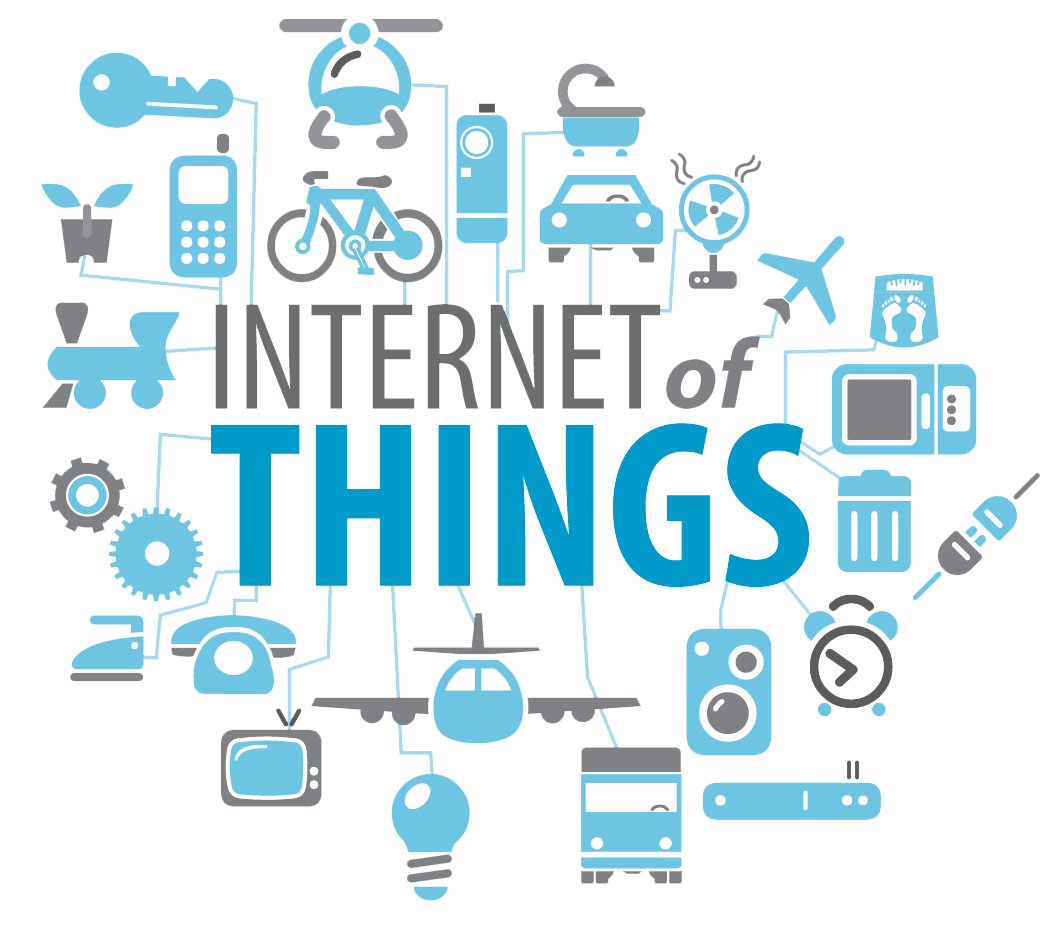
\includegraphics[width=0.9\textwidth]{images/iot}
    \label{fig:iot}
  \end{center}
\end{frame}

\begin{frame}{Grundlagen - Internet of Things}
  \Large
  \begin{itemize}
    \item Alltägliche Geräte
    \item Zugang zu IP-Netz
    \item Unterstützung des Menschen
  \end{itemize}

  \vspace{0.5cm}

  \begin{quote}
    \normalsize
    Das Ziel des \textbf{Internets der Dinge} ist es, die Informationslücke
    zwischen der realen und virtuellen Welt zu minimieren.
    \begin{flushright}
      \small
      -- Mattern, F. (2005), Das Internet der Dinge
    \end{flushright}
  \end{quote}
\end{frame}

\begin{frame}[fragile]
  \begin{center}
    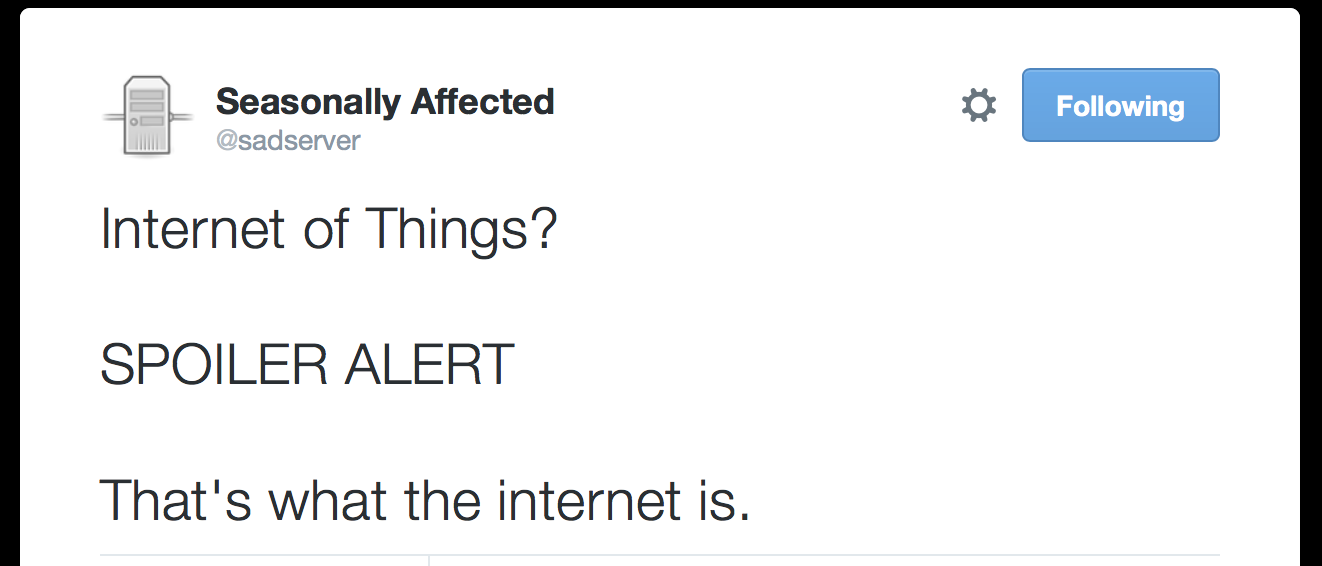
\includegraphics[width=0.75\textwidth]{images/sadserver1}
    \label{fig:spoiler}
  \end{center}
\end{frame}

\begin{frame}{Es ist nicht alles Gold}
  \begin{center}
    \begin{quote}
      Weder der Kühlschrank, noch das Fitness-Armband, noch die
      Waschmaschine sind \alert{aktive Elemente}. Sie übermitteln
      vielmehr nur die erfassten Daten an \alert{zentrale Stellen}.
      Dort werden die Daten analysiert, kombiniert, und entsprechende
      Reaktionen in die Wege geleitet:\\
      Die Lebensmittel-Bestellung tätigt nicht der Kühlschrank,
      sondern \alert{die Cloud}.
      \begin{flushright}
        -- Linus Neumann,\\
        \tiny
        \url{http://linus-neumann.de/wp-content/uploads/2015/10/Sensoren_der_Cloud.pdf}
      \end{flushright}
    \end{quote}
  \end{center}
\end{frame}
